%%%%%%%%%%%%%%%%%%%%%%%%%%%%%%%%%%%%%%%%%%%%%%%%%%%%%%%%%%%%%%%%%%%%%%%%%%%%%%%
%
% Tommy P. Keane
% Master of Science Thesis
% Department of Electrical and Microelectronic Engineering
%
% March 2011
%
%
%
% .tex and .sty modified from:
% http://www.ce.rit.edu/studentresources/gradresource/LaTexThesis.zip
%
%%%%%%%%%%%%%%%%%%%%%%%%%%%%%%%%%%%%%%%%%%%%%%%%%%%%%%%%%%%%%%%%%%%%%%%%%%%%%%%

%%%%%%%%%%%%%%%%%%%%%%%%%%%%%%%%%%%%%%%%%%%%%%%%%%%%%%%%%%%%%%%%%%%%%%%%%%%%%%%
%
% CHAPTER 2
%
% SECTION 3
%
%%%%%%%%%%%%%%%%%%%%%%%%%%%%%%%%%%%%%%%%%%%%%%%%%%%%%%%%%%%%%%%%%%%%%%%%%%%%%%%


%%%%%%%%%%%%%%%%%%%%%%%%%%%%%%%%%%%%%%%%%%%%%%%%%%%%%%%%%%%%%%%%%%%%%%%%%%%%%%%
% BEGIN DOCUMENT

A digital image histogram, referred to by $\textbf{h}(\textbf{n})$, is a discrete function whose dependent variable represents intensity value totals (counted) from the related digital image, and whose independent variable represents the index into the set of sub-ranges (bins) of intensities in the related digital image. The set of intensity values in the range subset is called the bin, having width r, as denoted by Eq. \ref{histBin}. And these independent variables, the range subset indices, are usually used interchangeably with referring to the bin centers. 

\begin{equation}
\label{histBin}
\left[n_{i}-\frac{r}{2},n_{i}+\frac{r}{2}\right)
\end{equation}

Thus, an intensity histogram is a vector holding the sums of intensity values in the sub-ranges. Harkening back to our assumption of images with 8-bits per pixel (8-bpp), this allows for a maximum of 256 unique intensity values per pixel per channel. And again these intensity values are assumed to be statistically random over the 2-D spatial domain of the image. So for a single channel image with 8-bpp a 256 bin histogram can be developed with integer width bins with a total range of $[0,255]$ and sub-ranges (bins): $[n_{i},n_{i+1})$. This histogram is again labeled $\textbf{h}(\textbf{n})$, with $n_{i} \epsilon \{\mathbb{Z}\}_{0}^{256}$, and mathematically the centers can be assumed to be at $\frac{n_{i+1}-n_{i}}{2}$ with width $r=1$, although in practice the half values are outside the 8-bpp intensity range. The total sum of that histogram, as shown in Eq. \ref{histSum}, is the product of the image dimensions, $\mathfrak{m} \cdot \mathfrak{n}$, provided the bins cover the full intensity range. (Note: histograms are defined as a one-to-one transformation of the image data, meaning that no pixel is counted in the histogram more than once)

\begin{equation}
\label{histSum}
	\mathfrak{m} \cdot \mathfrak{n} = \sum_{i=0}^{255}{h(n_{i})}
\end{equation}

As stated, any digital image histogram that covers the entire image and the entire intensity range will always sum to the image size, because all intensity values will fall in the range of the histogram bin intervals, by construction, and can only be counted once, by definition. This is how the PMF can be constructed; by normalizing a histogram by its sum total. The normalization will impose the constraint that an image�s intensity histogram�s sum will equal 1, which is a condition of a PMF; and clearly the histogram describes how many pixels correspond to an intensity value or range, which when normalized can be seen as a corollary to the probability of that intensity value or range occurring within the image. The specificity of the histogram to the image must be recognized though; because what the histogram conveys is that the pixels in \textit{this} image are distributed in \textit{these} amounts. Since an image is a single instance of a random function ($f(x,y)$), and a group of related random functions ($\{f_{1},f_{2},...\}$) should share an equivalent distribution described by their PMF, then a digital image histogram is not identical to a digital PMF, because it is a descriptor of a specific instance of a random function (the image) not a descriptor of the group of functions that this instance originated from. The imaging equivalence made here is that the normalized histogram is cognitively generalized to be a descriptor of the real-world scene that the related image (view�s frame) has captured. This is a very important point of consideration, but its detailed discussion has been deferred to the next section of this chapter and it should be taken for now as an assumption of this development.


After understanding what a histogram is and how to build it, its use is only as good as its limitations. And one of the most important limitations of an intensity histogram is the loss of spatial information in its generation. No spatial information is mathematically present in the calculation of a basic intensity histogram, as it has been described and used herein. However, through basic cognitive information relating to the structure and generation of images, there can be some basic yet significant spatial information extracted from a digital histogram. To illustrate this concept, Figure \ref{sampleHistogram} displays a very simple histogram for a 2-bpp image of size $3\times4$.

\begin{figure}
\label{sampleHistogram}
\centering
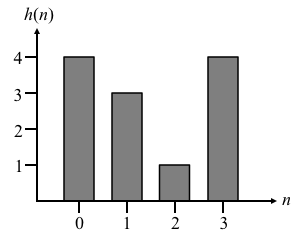
\includegraphics[width=.5\textwidth]{sampleHistogram}
\caption{Example Intensity Histogram}
\end{figure}

What is gathered from this histogram about the image is that there are equal numbers of extreme intensity values, and much more 1s than 2s (here the indices correspond to the intensity values as it is a full-range histogram). This results from a simple reading of the histogram and understanding its basic construction. But in terms of image information, it is also quite clear that this is a mostly dark image with high contrast. This comes from examining the values and structure of the histogram. The values are not bunched up nor are they spread evenly across intensities, so there are some significant edges in the image. Again, though, there is no explicit orientation information present in the mathematical construction of a histogram. Implicitly though this absolutely cannot be a smooth intensity gradient image, meaning that there is no way to construct these pixels with these values so that there is no edge with a transition greater than 1. Figure \ref{sampleImages} shows 4 unique images that all share the histogram shown in Figure \ref{sampleHistogram}.

\begin{figure}
\label{sampleImages}
\centering
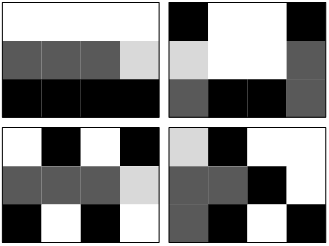
\includegraphics[width=.6\textwidth]{sampleImages}
\caption{Example 2-bpp Images with Identical Intensity Histograms (0 to 3 :: Black to White)}
\end{figure}

After looking at the images in Figure \ref{sampleImages}, the previous assertion becomes clear as there are always several intensity edges of value greater than 1. These images come from the set of 138,600 possible images ($\frac{12!}{4!\cdot4!\cdot3!\cdot1!}$) that share the histogram in Figure \ref{sampleHistogram}. But this is just a mathematical example with no constraints. By the nature of reality, such as the spatial and temporal continuity of objects within reality, images of real scenes are highly constrained subset of all the possible images from the total set (all the possible combinations of intensities given the number of pixels in the image). Any 2-bpp image of size $3\times4$ is actually in a set of $4^{12}$ images, and so the set of images with the histogram in Figure \ref{sampleImages} is roughly less than $0.8\%$ of the total set, while still unconstrained to real world shapes. Thus real world images, constrained by relatively similar histograms, are in an even smaller subset, most likely in the range of $0.05\%$, with a conservative factor of 10 estimate. For example, the images used in this algorithm were all roughly of the size $480 \times 640$ and were 3 channel images of 8-bpp, giving 768 possible values per pixel. This shows that there are $768^{480\cdot640}$ possible images with no spatial or histogram constraint. Any histogram, color constancy model, texture, object contiguity, or any other real world aspect or feature relevant to the digital image will create a smaller and smaller subset. Again, just looking at the previous equation used to calculate the histogram based subset, reapplied in Eq.s \ref{combinatorics} and \ref{bitDepth}, there is a significant decrease in variability.


\begin{equation}
\label{combinatorics}
	\frac{\mathfrak{p} \cdot \left(\mathfrak{m} \cdot \mathfrak{n}\right)!}{ \prod_{i}{\left(n_{i}^{(R)}!\right)} \cdot \prod_{j}{\left(n_{j}^{(G)}!\right)} \cdot \prod_{k}{\left(n_{k}^{(B)}!\right)} }
\end{equation}

\begin{equation}
\label{bitDepth}
	\left( 3 \cdot 2^{b} \right)^{\left(\mathfrak{m} \cdot \mathfrak{n}\right)}
\end{equation}

A rigorous mathematical comparison is not applicable here, but looking at Eq. \ref{combinatorics} compared to Eq. \ref{bitDepth}, it is clear that Eq. \ref{bitDepth} is a monotonically increasing exponential with $\mathfrak{m}$ and $\mathfrak{n}$ while Eq. \ref{combinatorics} is clearly varying with respect to the product of the products in the denominator. The more repetition there is in the given histograms the faster Eq. \ref{combinatorics} will decrease from its already smaller factorial value (compared to the exponential of Eq. \ref{bitDepth}). Again a rigorous discussion is beyond the scope of this work because the purpose here is to illuminate how small the subset of all possible real world images is, and how much smaller the set of all similar images is, and how much smaller the set of similar real world images with similar histograms is. There are several layers of constriction creating such a small subset that clearly the approximation of using a normalized histogram to produce a so-called digital image PDF is a theoretically relevant and a quite realistic simplification. Conceptually what is being stated or assumed is that when viewing the same scene two different views will be essentially sampling the same random function, meaning that they should be describable by the same image PDF. As the overlap decreases between the views the image PDF will be less and less applicable.


This is a direct extension into the WFMI algorithm�s matching scheme and metric calculation. For a large enough image taken from a view that is capturing a scene, there should be enough structure and entropy within the image resultant from the scene (i.e. not just noise) that would allow for another image captured from another view of the scene to share similar data. There will certainly intensity variations, noise concerns, and the data variation coming from occlusion and parallax differences between the views. However, the subsets (regions) of the images that correspond to the same subsets (regions or segments) of the scene should share a similar distribution, or should be accurately conceptually characterized as sharing the same image PDF, in that region. If the images are too small or the region is chosen to be too small, this extension will fail. This can follow mathematically, albeit not presented rigorously here, from Eq.s \ref{combinatorics} and \ref{bitDepth}. As m and n decrease there is less opportunity for variation or consistency in the image, depending upon the value of b. If $2^{b}$ is significant compared to $\mathfrak{m} \cdot \mathfrak{n}$ then each instance of an image from that theoretical set will have significant variation, even when the views are capturing the same scene or sections of the views are capturing the same scene. This is a crippling limit of these assumptions and a source of our empirically derived overlap requirement for the algorithm, as discussed in Chapter 4.


These are extremely important characteristics to understand about intensity histograms. Of course a histogram could be extended to be a spatio-intensity histogram, which would make it a 4-D function with 3 independent variables from the two spatial image axes and the intensity value. But in each channel there is only one pixel at location $\left(0,0\right)$ and that pixel has only one intensity value per channel. The histogram should be seen almost as a projection of the intensity data of the image from the spatial coordinates into a single intensity coordinate. If the spatial information would be considered a full-range spatio-intensity histogram of an m?n?1 image would be the image itself. Significant bin sizes would be needed in the spatial dimensions, but this could be seen as equivalent to finding block-based or region-based histograms, so a definition as such would just be adding unnecessary nomenclature. Also it will be discussed in Chapter 3 as to how computationally taxing the histogram calculation is, and expanding it is a significant detriment to the algorithm. But in considering the assumptions made thus far, note that if spatial information were added into a histogram (especially full-range spatial dependence) the significant occlusions or variations in parallax of the views of the scene would generate very different histograms. Under this scenario, assuming that these different views can be modeled by the same (or in practice, a similar) distribution will be entirely false and misleading. Any image PDF based metric (such as mutual information) will generate a sparse correspondence map because the noise, illumination variations, and scene geometry variations will never align in the same spatial location within the frames from the various views. Avoiding spatial information in the calculation of the image distribution (PDF) is an essential factor in generating a robust algorithm and pushes the results towards conceptual accuracy rather than digital accuracy, as following the model of the trained observer viewing multiple surveillance feeds.


This all follows directly into the generation of, and ambiguities inherent to, mutual information calculations of digital images. So first it is necessary to take a similar look at the calculation of mutual information, and what it can and will represent in this context.


%%%%%%%%%%%%%%%%%%%%%%%%%%%%%%%%%%%%%%%%%%%%%%%%%%%%%%%%%%%%%%%%%%%%%%%%%%%%%%%
% END OF DOCUMENT

